\chapter{Identification hadronique dans le SDHCAL par apprentissage supervisé}
\label{sec:pid_mlp}

\section{Problématique physique et stratégie générale}

L’identification des particules hadroniques constitue un enjeu central pour l’exploitation des calorimètres hautement granulaires. Dans un détecteur tel que le SDHCAL, la structure fine des gerbes contient en principe suffisamment d’information pour distinguer plusieurs espèces hadroniques, en particulier les pions \(\pi^-\), les protons \(p\) et les kaons neutres longs \(K^0_L\). Une telle séparation est importante non seulement pour la classification des événements, mais aussi pour la reconstruction de l’énergie, puisque la réponse calorimétrique dépend de l’espèce incidente. Elle s’inscrit plus largement dans la logique des approches de type \emph{Particle Flow}, où la qualité de la reconstruction globale repose sur une identification correcte des objets détectés.

La difficulté provient de la nature même des interactions hadroniques. Contrairement aux gerbes électromagnétiques, dont le développement est relativement régulier, les gerbes hadroniques présentent de fortes fluctuations d’un événement à l’autre. Le point de première interaction, la profondeur moyenne de développement, l’étalement transverse, la densité locale des dépôts et la fraction d’énergie invisible varient sensiblement, même à énergie incidente fixée. Certaines espèces, comme les protons et les pions chargés, peuvent ainsi produire des signatures partiellement recouvrantes dans le calorimètre, rendant leur séparation non triviale.

Le SDHCAL possède néanmoins plusieurs caractéristiques particulièrement favorables à cette tâche. Sa très haute granularité permet de reconstruire la morphologie des gerbes couche par couche, tandis que la lecture semi-digitale à trois seuils apporte une information indirecte sur la densité locale du dépôt d’énergie. Lorsqu’une information temporelle est disponible, elle peut également contribuer à la discrimination via le temps de vol ou la dynamique d’initiation de la gerbe. L’ensemble forme un espace d’observables riche, mais complexe, dans lequel les corrélations entre variables jouent un rôle important.

Dans ce contexte, une approche par apprentissage supervisé s’impose naturellement. Les descripteurs extraits sont nombreux, souvent corrélés et leur pouvoir discriminant repose sur des dépendances non linéaires difficiles à exploiter au moyen de simples coupures séquentielles. L’objectif est donc d’entraîner un classificateur capable d’apprendre automatiquement une frontière de séparation efficace entre les différentes espèces hadroniques à partir de leur signature calorimétrique.

Plusieurs familles de modèles ont été étudiées dans ce travail, notamment des perceptrons multicouches, des forêts aléatoires et des arbres de décision boostés. Les meilleurs résultats ayant été obtenus avec cette dernière catégorie, nous retenons finalement une implémentation de type LightGBM comme modèle de référence pour la classification multiclasse des particules \(\pi^-\), \(p\) et \(K^0_L\).

\section{Données simulées et descripteurs physiques}

L’étude repose sur des échantillons simulés de particules mono-énergétiques correspondant aux trois espèces hadroniques considérées : pions négatifs \(\pi^-\), protons \(p\) et kaons neutres longs \(K^0_L\). Chaque classe contient environ \(1.3\times10^{5}\) événements, générés dans une gamme d’énergie comprise entre 1 et 130~GeV. Ce domaine couvre à la fois les interactions de basse énergie, où les gerbes restent peu développées, et les régimes plus énergétiques, caractérisés par une activité hadronique plus étendue et plus fluctuante.

Un prétraitement initial est appliqué afin de ne conserver que les événements valides associés aux codes PDG d’intérêt. Les hits enregistrés dans le SDHCAL sont ensuite convertis en observables globales décrivant la gerbe incidente. Lorsque l’étude inclut l’information temporelle, un smearing gaussien peut être appliqué afin de reproduire une résolution instrumentale réaliste. Les détails techniques complets de la préparation des données sont regroupés en Annexe~\ref{app:pid_data}.

Plutôt que d’utiliser directement la liste exhaustive des hits du détecteur, nous construisons un ensemble de descripteurs physiques résumant les principales propriétés morphologiques de chaque événement. Ces variables sont extraites à l’aide de l’outil \texttt{ShowerAnalyzer}, développé en \texttt{C++}, puis utilisées comme entrées des algorithmes de classification.

Les observables retenues peuvent être regroupées en plusieurs familles complémentaires :

\begin{itemize}
    \item \textbf{Activité globale et information en seuils :} nombre total de hits, occupations associées aux trois seuils semi-digitaux (\texttt{Thr1}, \texttt{Thr2}, \texttt{Thr3}), multiplicité locale. Ces variables renseignent sur l’intensité globale de la gerbe et sur la densité locale des dépôts d’énergie.

    \item \textbf{Développement longitudinal :} plan de début de gerbe (\texttt{Begin}), barycentre en profondeur (\texttt{Zbary}), dispersion longitudinale (\texttt{Zrms}), position du maximum ou paramètres ajustés du profil longitudinal. Elles sont sensibles à la profondeur de première interaction et à l’évolution de la cascade dans l’absorbeur.

    \item \textbf{Développement transverse et compacité :} rayon effectif (\texttt{Radius}), densité locale (\texttt{Density}), excentricité, valeurs propres géométriques (\texttt{\(\lambda_1\)}, \texttt{\(\lambda_2\)}). Ces observables décrivent l’étalement latéral et l’anisotropie spatiale de la gerbe.

    \item \textbf{Structure locale :} nombre de clusters intra-couche, taille moyenne et maximale des clusters, présence éventuelle de segments quasi-linéaires. Elles caractérisent la fragmentation interne de l’activité.

    \item \textbf{Variables temporelles :} temps du premier hit (\texttt{tMin}), temps moyen (\texttt{tMean}), dispersion temporelle (\texttt{tSpread}). Elles peuvent refléter à la fois le temps de vol de la particule incidente et la dynamique temporelle de l’interaction hadronique.
\end{itemize}

L’utilisation conjointe de ces différentes familles vise à exploiter l’ensemble de l’information accessible dans le SDHCAL. Certaines variables décrivent principalement la géométrie de la gerbe, d’autres son intensité locale ou sa chronologie. Leur combinaison fournit ainsi une représentation compacte, mais physiquement pertinente, de chaque événement.

La définition détaillée des observables utilisées est présentée en Annexe~\ref{annexe:showeranalyzer}, où figure également un tableau récapitulatif complet (Table~\ref{tab:recap_features}).

\section{Comparaison des modèles et choix de LightGBM}

Plusieurs approches d’apprentissage supervisé ont été étudiées afin d’identifier la méthode la plus adaptée à la classification des particules hadroniques dans le SDHCAL. L’objectif n’était pas uniquement de maximiser la performance brute, mais également de rechercher un compromis satisfaisant entre pouvoir discriminant, robustesse statistique, temps d’entraînement et capacité à traiter efficacement des variables tabulaires hétérogènes.

Trois grandes familles de modèles ont été comparées :

\begin{itemize}
    \item \textbf{Perceptron multicouche (MLP) :} réseau de neurones dense capable d’apprendre des relations non linéaires complexes entre les variables d’entrée. Ce type d’architecture est flexible, mais requiert généralement un réglage plus fin des hyperparamètres (profondeur, largeur, régularisation, optimisation) et se montre plus sensible au prétraitement des variables.

    \item \textbf{Forêt aléatoire (Random Forest) :} ensemble d’arbres de décision indépendants entraînés sur des sous-échantillons aléatoires des données. Cette approche est robuste, simple à mettre en œuvre et peu sensible aux transformations des variables, mais peut perdre en efficacité lorsque la frontière de séparation entre classes nécessite la combinaison progressive de nombreux critères faibles.

    \item \textbf{Arbres de décision boostés (BDT) :} succession d’arbres faibles construits itérativement, chaque nouvel arbre cherchant à corriger les erreurs des précédents. Cette stratégie est particulièrement performante pour les jeux de données tabulaires structurés présentant corrélations, non-linéarités et interactions complexes entre variables.
\end{itemize}

Les comparaisons préliminaires réalisées sur un même jeu de variables d’entrée ont montré que les méthodes de boosting fournissaient les meilleures performances globales pour la séparation des classes \(\pi^-\), \(p\) et \(K^0_L\). Elles se sont révélées plus précises que les forêts aléatoires, tout en nécessitant moins d’ajustements fins qu’un réseau de neurones dense.

Au sein de cette famille, nous avons retenu l’implémentation \textbf{LightGBM} (\emph{Light Gradient Boosting Machine}) \cite{ke2017}. Ce choix repose sur plusieurs avantages pratiques et méthodologiques :

\begin{itemize}
    \item excellentes performances sur les jeux de données tabulaires de grande taille ;
    \item prise en compte naturelle des relations non linéaires entre variables ;
    \item bonne robustesse face aux corrélations et aux variables de nature différente ;
    \item temps d’entraînement réduit grâce à une implémentation optimisée ;
    \item accès direct à des indicateurs d’importance des variables, utiles pour l’interprétation physique.
\end{itemize}

Ce dernier point présente un intérêt particulier dans le cadre de cette étude. Au-delà de la seule performance prédictive, il est essentiel d’identifier quelles observables du détecteur contribuent le plus à la séparation des espèces. Les méthodes de boosting offrent ainsi un compromis particulièrement pertinent entre efficacité, rapidité et interprétabilité.

En pratique, LightGBM a offert le meilleur équilibre entre précision, stabilité numérique et coût de calcul. Ces résultats justifient son adoption comme modèle de référence pour la classification multiclasse des particules hadroniques dans la suite de ce travail.

\section{Stratégie d'entraînement et métriques}

Afin d’évaluer de manière rigoureuse les performances du classificateur, le jeu de données complet est séparé en trois sous-ensembles indépendants : un ensemble d’entraînement, un ensemble de validation et un ensemble de test. Le découpage est réalisé de manière stratifiée, de façon à conserver des proportions comparables de pions \(\pi^-\), de protons \(p\) et de kaons neutres longs \(K^0_L\) dans chacun des sous-échantillons.

L’ensemble d’entraînement est utilisé pour ajuster les paramètres internes du modèle. L’ensemble de validation intervient au cours de l’apprentissage afin de suivre les performances sur des données non vues et de guider le réglage des hyperparamètres. Enfin, l’ensemble de test, totalement exclu des étapes précédentes, est réservé à l’évaluation finale du classificateur. Cette séparation garantit une estimation non biaisée de la capacité de généralisation du modèle.

Le modèle LightGBM est entraîné en mode multiclasse à l’aide d’une fonction de coût de type \emph{multi-logloss}. Cette quantité mesure l’écart entre les probabilités prédites par le modèle et les classes réelles. Sa minimisation favorise à la fois des prédictions correctes et des probabilités bien calibrées. Pour un problème comportant \(K\) classes et \(N\) événements, elle s’écrit :

\[
\mathcal{L}
=
-\frac{1}{N}
\sum_{i=1}^{N}
\sum_{k=1}^{K}
y_{ik}\,\log p_{ik},
\]

où \(y_{ik}=1\) si l’événement \(i\) appartient à la classe \(k\) (et \(0\) sinon), tandis que \(p_{ik}\) désigne la probabilité prédite correspondante.

Afin de limiter le sur-apprentissage, un mécanisme d’arrêt anticipé (\emph{early stopping}) est mis en œuvre. L’apprentissage est interrompu lorsque la performance sur l’ensemble de validation cesse de s’améliorer après un nombre donné d’itérations consécutives. Cette procédure permet de retenir automatiquement une complexité optimale du modèle, sans dégrader sa capacité de généralisation.

Des tests exploratoires de rééquilibrage des classes ont également été réalisés, notamment via la méthode \emph{SMOTE} (\emph{Synthetic Minority Over-sampling Technique}). Les gains observés sont toutefois restés limités dans la configuration étudiée. De plus, la génération d’événements synthétiques peut introduire des corrélations artificielles ou modifier localement la structure statistique des données. Pour ces raisons, cette stratégie n’a pas été retenue dans la chaîne principale ; les détails correspondants sont présentés en annexe.

Les performances finales sont ensuite quantifiées à l’aide de plusieurs métriques complémentaires :

\begin{itemize}
    \item \textbf{Accuracy globale :} fraction totale d’événements correctement classés ;

    \item \textbf{Accuracy équilibrée :} moyenne des taux de bonne classification par classe, moins sensible à d’éventuels déséquilibres statistiques ;

    \item \textbf{Matrice de confusion :} répartition détaillée des prédictions entre classes vraies et classes reconstruites, particulièrement utile pour identifier les ambiguïtés dominantes ;

    \item \textbf{Multi-logloss :} indicateur sensible à la qualité probabiliste des prédictions ;

    \item \textbf{Courbes ROC one-vs-rest et aire sous la courbe (AUC) :} métriques évaluant la capacité de séparation de chaque classe vis-à-vis des autres à seuil variable ;

    \item \textbf{Histogrammes des probabilités prédites :} distributions des scores de sortie du modèle, permettant d’évaluer le degré de séparation effectif entre espèces.
\end{itemize}

L’utilisation conjointe de ces métriques est essentielle. Une accuracy élevée ne garantit pas nécessairement une bonne calibration probabiliste, tandis qu’une matrice de confusion permet d’identifier précisément quelles espèces restent difficiles à distinguer. De même, les courbes ROC et les valeurs d’AUC apportent une vision plus robuste du pouvoir séparateur du classificateur que la seule performance globale.

Dans le cadre présent, la confusion résiduelle entre protons et pions constitue ainsi un indicateur plus informatif que l’accuracy seule.

Les détails numériques relatifs au découpage des données, aux hyperparamètres retenus et aux réglages techniques utilisés pour l’entraînement sont rassemblés en Annexe~\ref{app:pid_hyperparams}.

\section{Résultats de classification}

Les performances du modèle LightGBM sont évaluées sur l’ensemble de test indépendant, non utilisé lors des phases d’apprentissage et de validation. Les résultats présentés ci-dessous reflètent donc la capacité réelle de généralisation du classificateur pour la séparation des trois espèces hadroniques étudiées : pions négatifs $\pi^-$, protons $p$ et kaons neutres longs $K^0_L$.

\paragraph{Évolution de l’apprentissage.}

La Figure~\ref{fig:train-curve} présente l’évolution de la fonction de coût \emph{multi-logloss} au cours de l’entraînement, pour les ensembles d’apprentissage et de validation. Les deux courbes décroissent de manière régulière et restent proches l’une de l’autre sur l’ensemble des itérations.

La perte de validation se stabilise autour de $\sim 0.61$, sans divergence marquée vis-à-vis de la courbe d’entraînement. Ce comportement indique un apprentissage stable, sans signe important de sur-ajustement. L’arrêt anticipé permet ainsi de retenir un compromis satisfaisant entre performance et capacité de généralisation.

\begin{figure}[!ht]
  \centering
  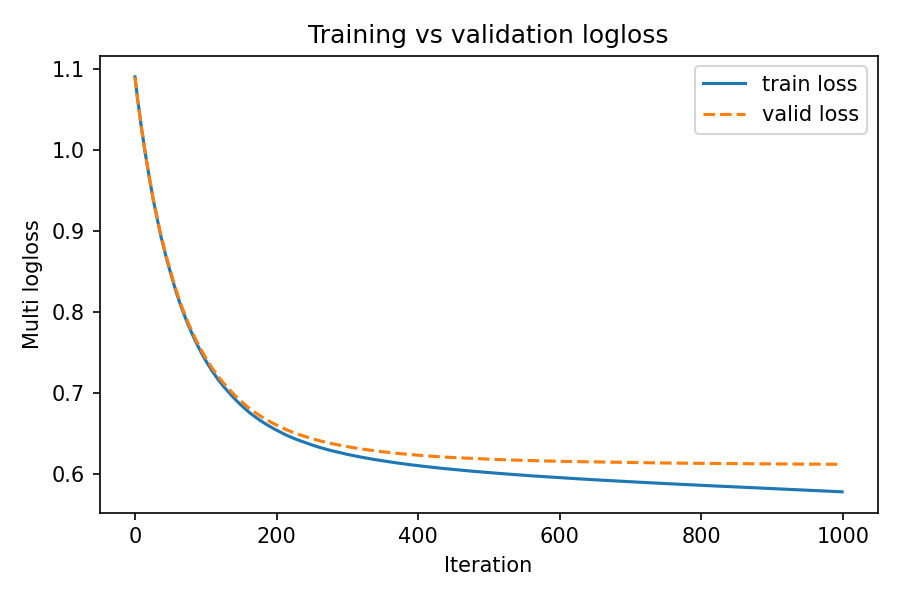
\includegraphics[width=0.50\linewidth]{Fig/training_curve_9.png}
  \caption{Évolution de la fonction de coût \textit{multi-logloss} sur les ensembles d’entraînement et de validation au cours de l’apprentissage LightGBM.}
  \label{fig:train-curve}
\end{figure}

\paragraph{Matrice de confusion.}

La matrice de confusion normalisée obtenue sur l’échantillon de test est représentée Figure~\ref{fig:cm}. Elle met en évidence des comportements sensiblement différents selon les espèces considérées et fournit une information plus riche que la seule accuracy globale.

\begin{itemize}
    \item \textbf{Pions $\pi^-$} : environ $48.8\,\%$ des événements sont correctement identifiés, tandis que $\sim47.9\,\%$ sont confondus avec des protons. La reconnaissance des pions constitue ainsi la principale difficulté du problème étudié.

    \item \textbf{Protons $p$} : la séparation est meilleure, avec $\sim68.6\,\%$ d’identifications correctes. L’erreur dominante correspond à une attribution erronée vers la classe pion ($\sim27.4\,\%$).

    \item \textbf{Kaons neutres $K^0_L$} : la classification est nettement plus performante, avec environ $86.0\,\%$ des événements correctement reconstruits, ce qui traduit une signature calorimétrique plus spécifique.
\end{itemize}

En supposant des classes de tailles comparables, ces résultats correspondent à une \textbf{accuracy globale} d’environ $68\,\%$. Cette valeur doit toutefois être interprétée avec prudence : elle traduit un niveau de performance global satisfaisant pour un problème hadronique multiclasse non trivial, mais masque des disparités importantes entre classes.

Le résultat le plus marquant n’est donc pas tant la valeur moyenne de l’accuracy que la structure des erreurs observées. La confusion massive entre pions et protons indique que ces deux espèces occupent des régions partiellement recouvrantes dans l’espace des variables utilisées, tandis que les $K^0_L$ se distinguent beaucoup plus nettement.

Cette dissymétrie justifie l’usage de métriques complémentaires telles que les rappels par classe, l’accuracy équilibrée ou les courbes ROC one-vs-rest, mieux adaptées pour caractériser finement les performances d’un classificateur multiclasse.

\begin{figure}[!ht]
  \centering
  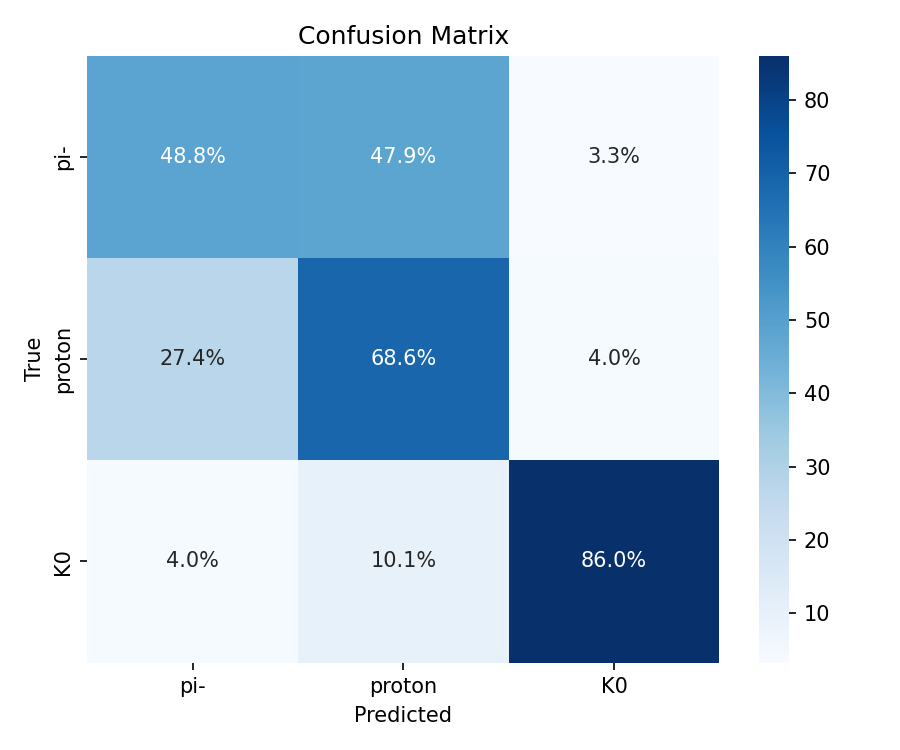
\includegraphics[width=0.50\linewidth]{Fig/confusion_matrix_9.png}
  \caption{Matrice de confusion normalisée (pourcentages par ligne). Les classes sont ordonnées selon \{$\pi^-$, $p$, $K^0_L$\}.}
  \label{fig:cm}
\end{figure}

\paragraph{Interprétation physique.}

La meilleure séparation observée pour les $K^0_L$ s’explique principalement par une dynamique hadronique différente de celle des pions et des protons, qui se répercute directement sur la morphologie des gerbes mesurées dans le SDHCAL.

Dans les interactions hadroniques se produisant dans l’absorbeur, les états finaux sont très souvent dominés par la production de pions. Ce comportement résulte conjointement :

\begin{itemize}
    \item de la faible masse des pions, qui les rend énergétiquement faciles à produire ;
    \item des symétries approximatives de l’interaction forte, notamment liées à l’isospin ;
    \item d’un espace de phase plus favorable ;
    \item de l’absence de création de quarks étranges supplémentaires.
\end{itemize}

À l’inverse, la production de kaons nécessite la création d’étrangeté (\(s\bar{s}\)) et implique des masses plus élevées. Elle est donc statistiquement moins probable aux énergies considérées ici. Les hadrons contenant de l’étrangeté, comme les $K^0_L$, présentent ainsi des modes d’interaction et des cascades secondaires en moyenne différents de ceux dominés par les pions.

Un rôle important est également joué par la production de mésons neutres $\pi^0$, qui se désintègrent quasi instantanément selon :

\[
\pi^0 \rightarrow \gamma\gamma.
\]

Ils alimentent alors la composante électromagnétique de la gerbe. Les fluctuations du nombre de $\pi^0$ produits influencent directement la compacité locale, la densité d’activité et le développement longitudinal observés dans le calorimètre. Les différences statistiques de production de ces composantes entre espèces contribuent donc au pouvoir discriminant du classificateur.

Les $K^0_L$ tendent ainsi à générer des signatures calorimétriques plus spécifiques, ce qui explique leur meilleure séparation expérimentale.

À l’inverse, les protons et les pions chargés présentent des comportements plus proches. Tous deux interagissent via l’interaction forte sans nécessiter de dynamique d’étrangeté, et leurs gerbes restent largement dominées par les fluctuations de première interaction nucléaire ainsi que par la variabilité de la composante électromagnétique secondaire. Il en résulte un recouvrement important dans l’espace des variables tabulaires utilisées ici, rendant leur frontière de séparation plus difficile à apprendre.

La confusion résiduelle pion/proton ne traduit donc pas une faiblesse particulière du modèle, mais reflète avant tout la proximité physique réelle de leurs signatures hadroniques dans le SDHCAL.

\paragraph{Probabilités prédites.}

Les histogrammes des probabilités de sortie du modèle (Figure~\ref{fig:hists}) confirment les tendances mises en évidence par la matrice de confusion et apportent une information complémentaire sur le degré de confiance des prédictions.

Les vrais $K^0_L$ reçoivent majoritairement des probabilités élevées pour leur classe correcte, avec une superposition limitée avec les distributions associées aux pions et aux protons. Cette séparation nette indique que le modèle identifie, pour une large fraction des événements, des signatures caractéristiques propres aux kaons neutres longs.

En revanche, les probabilités associées à la classe proton présentent un recouvrement significatif entre vrais protons et vrais pions. Une fraction non négligeable des événements des deux classes reçoit des scores intermédiaires, traduisant une zone d’ambiguïté où la décision du classificateur devient moins robuste.

Ce comportement est cohérent avec la proximité physique des signatures pion/proton dans le détecteur : pour certains événements, les observables de gerbe ne permettent pas une discrimination franche, même pour un modèle performant. La confusion observée ne provient donc pas uniquement de limites algorithmiques, mais également d’un recouvrement intrinsèque entre classes dans l’espace des variables utilisées.

Ces distributions suggèrent enfin qu’une exploitation probabiliste des sorties du modèle (seuils ajustés, calibration des scores, sélection d’événements de haute pureté) pourrait constituer une piste intéressante selon les besoins d’analyse.

\begin{figure}[!ht]
  \centering
  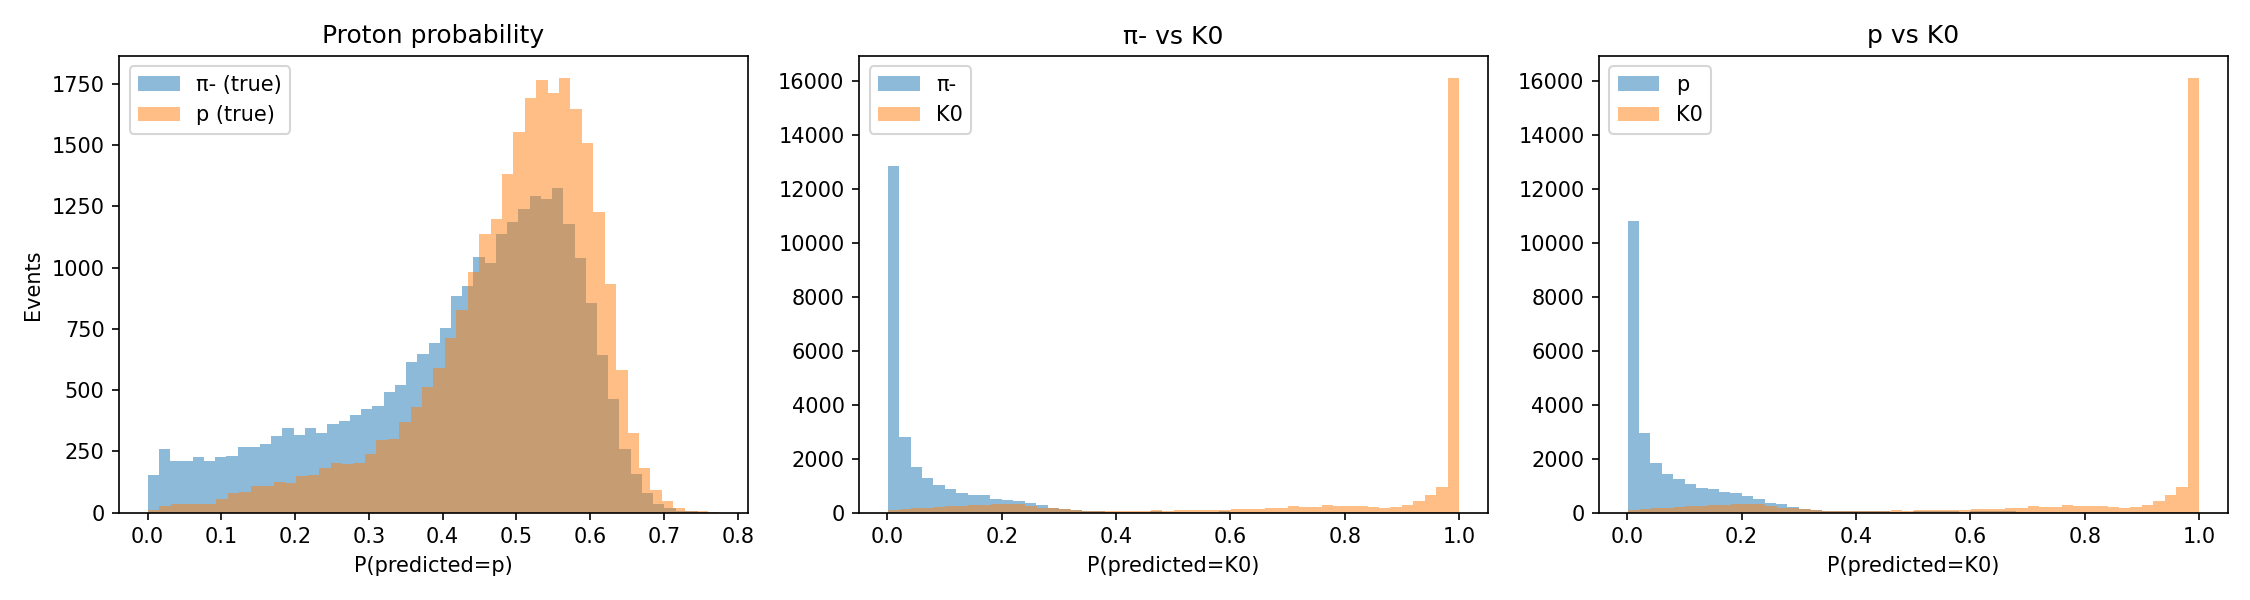
\includegraphics[width=\linewidth]{Fig/prob_hists_9.png}
  \caption{Histogrammes des probabilités prédites : (gauche) $P(\mathrm{classe}=p)$ pour vrais $\pi^-$ et vrais $p$ ; (centre) $P(\mathrm{classe}=K^0)$ pour vrais $\pi^-$ et vrais $K^0_L$ ; (droite) $P(\mathrm{classe}=K^0)$ pour vrais $p$ et vrais $K^0_L$.}
  \label{fig:hists}
\end{figure}

\paragraph{Bilan.}

Le classificateur LightGBM fournit ainsi une base solide pour l’identification hadronique tabulaire dans le SDHCAL. La séparation des $K^0_L$ apparaît robuste et bien maîtrisée, tandis que la confusion résiduelle entre protons et pions constitue la principale limitation actuelle du problème étudié.

L’accuracy globale d’environ $68\,\%$ doit ainsi être interprétée comme le résultat d’un compromis entre une excellente reconnaissance des $K^0_L$ et une séparation plus délicate du couple pion/proton, physiquement plus proche. Cette lecture détaillée est plus informative que la seule performance moyenne.

Ces observations motivent à la fois l’étude approfondie des variables discriminantes, l’usage de métriques par classe, ainsi que l’exploration de représentations plus fines des gerbes, notamment fondées directement sur les hits du détecteur.

\subsection{Corrélations et variables discriminantes}
\label{subsec:corr-perm}

Au-delà des performances globales du classificateur, il est important d’identifier quelles observables portent l’information la plus utile pour la séparation des particules. Cette analyse poursuit un double objectif : mieux comprendre les mécanismes physiques exploités par le modèle et repérer d’éventuelles redondances entre variables d’entrée.

Deux approches complémentaires ont été retenues :
\begin{itemize}
    \item l’étude des corrélations linéaires entre variables, à l’aide de la matrice de corrélation de Pearson ;
    \item l’analyse des importances internes du modèle LightGBM, estimées ici à partir du \emph{gain} cumulé apporté par chaque variable lors des coupures successives.
\end{itemize}

\paragraph{Matrice de corrélation.}

La Figure~\ref{fig:corr-matrix} présente la matrice de corrélation calculée sur l’ensemble des événements. Plusieurs groupes cohérents apparaissent naturellement.

\begin{itemize}
    \item \textbf{Activité globale et compacité de gerbe :} les variables \texttt{Thr1}, \texttt{Thr2}, \texttt{Thr3}, \texttt{NClusters}, \texttt{Nmax}, \texttt{AvgClustSize}, \texttt{MaxClustSize} et \texttt{Density} présentent des corrélations modérées à fortes. Cette structure est attendue, car ces observables mesurent toutes, sous des formes différentes, l’intensité locale ou globale de la gerbe.

    \item \textbf{Développement longitudinal :} \texttt{Begin}, \texttt{Zbary}, \texttt{Zrms}, \texttt{Xmax} et \texttt{z0\_fit} sont positivement corrélées. Elles décrivent conjointement la position de départ et l’évolution de la gerbe dans la profondeur du calorimètre.

    \item \textbf{Forme géométrique :} \texttt{\(\lambda_1\)}, \texttt{\(\lambda_2\)} et \texttt{eccentricity3D} apparaissent liées, ce qui reflète leur rôle commun dans la description de l’anisotropie spatiale.

    \item \textbf{Variables temporelles :} \texttt{tMin}, \texttt{tMean} et \texttt{tSpread} sont faiblement à modérément corrélées entre elles. Elles montrent également certains liens avec les variables longitudinales, suggérant une connexion entre chronologie du signal et profondeur d’initiation de la gerbe.
\end{itemize}

\begin{figure}[!ht]
  \centering
  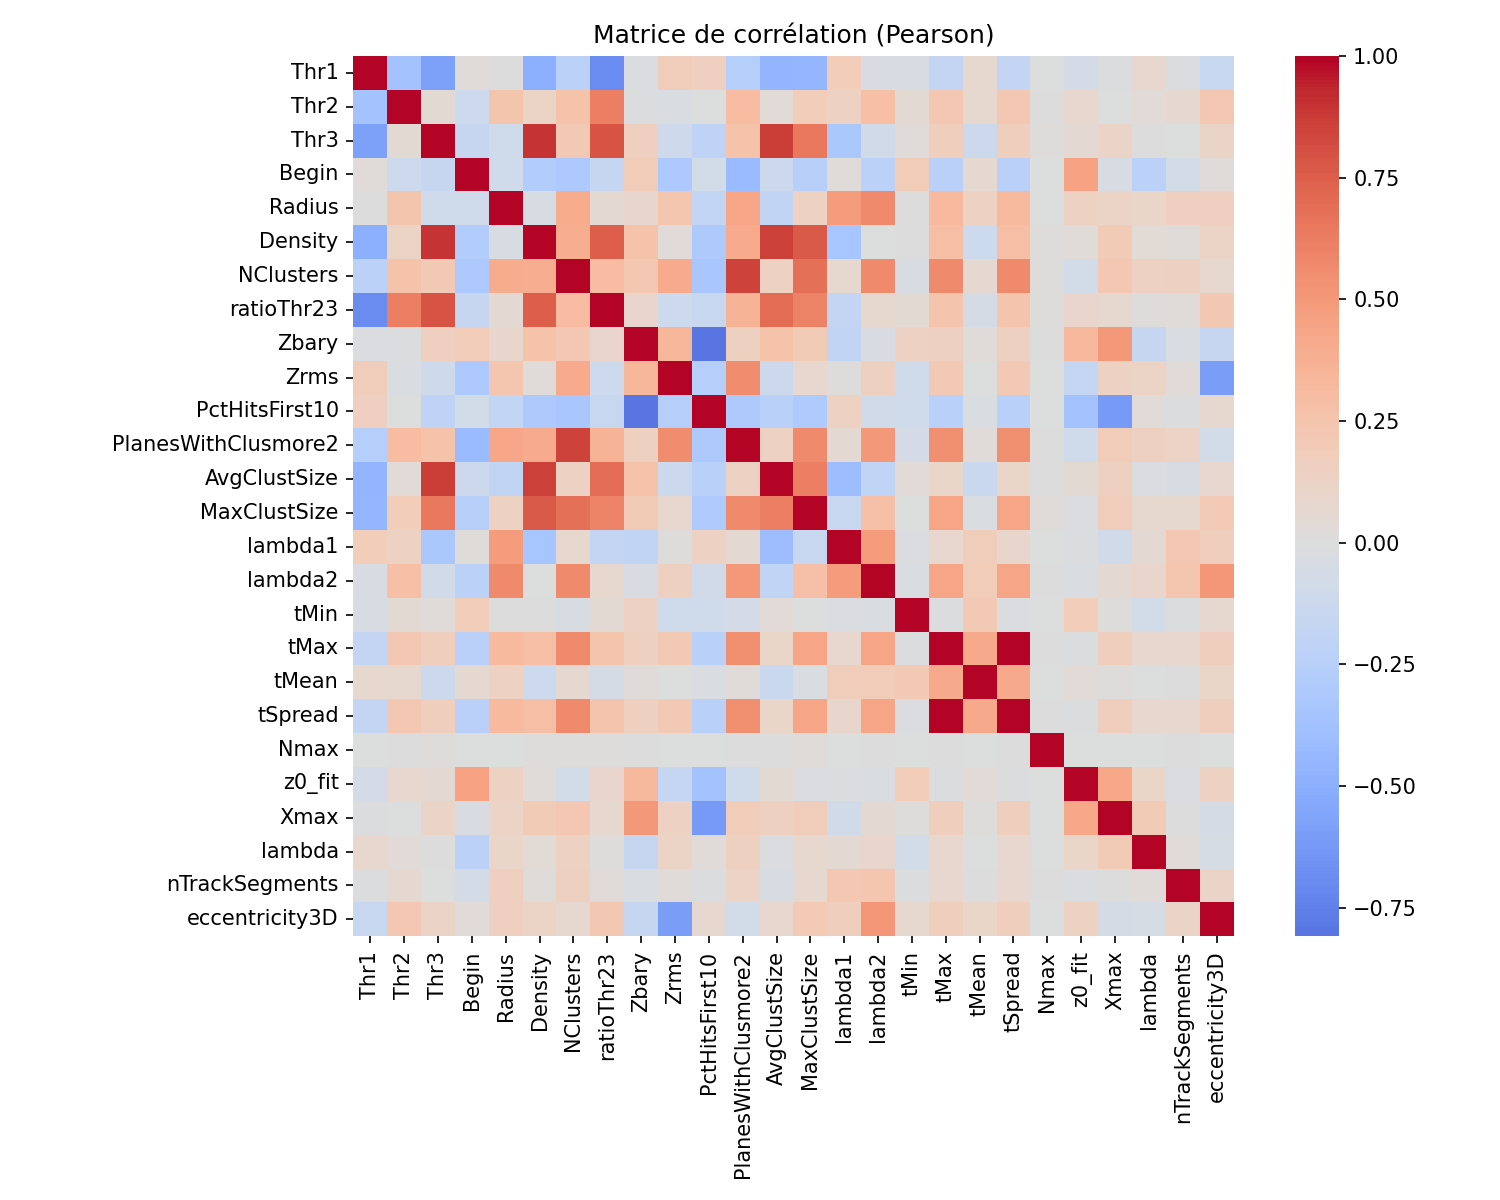
\includegraphics[width=0.75\linewidth]{Fig/correlation_matrix.png}
  \caption{Matrice de corrélation de Pearson des variables d’entrée utilisées pour la classification.}
  \label{fig:corr-matrix}
\end{figure}

Dans l’ensemble, cette organisation indique que plusieurs variables transportent une information partiellement redondante. Une sélection plus compacte des observables pourrait donc être envisagée sans perte majeure de performance.

\paragraph{Importances des variables dans LightGBM.}

La Figure~\ref{fig:perm-imp} présente les importances des variables estimées à partir du \emph{gain} cumulé de LightGBM. Cette quantité mesure la contribution totale de chaque variable à la réduction de la fonction de coût au cours de l’entraînement. Elle fournit ainsi une indication directe des observables les plus exploitées par le classificateur.

\begin{figure}[!ht]
  \centering
  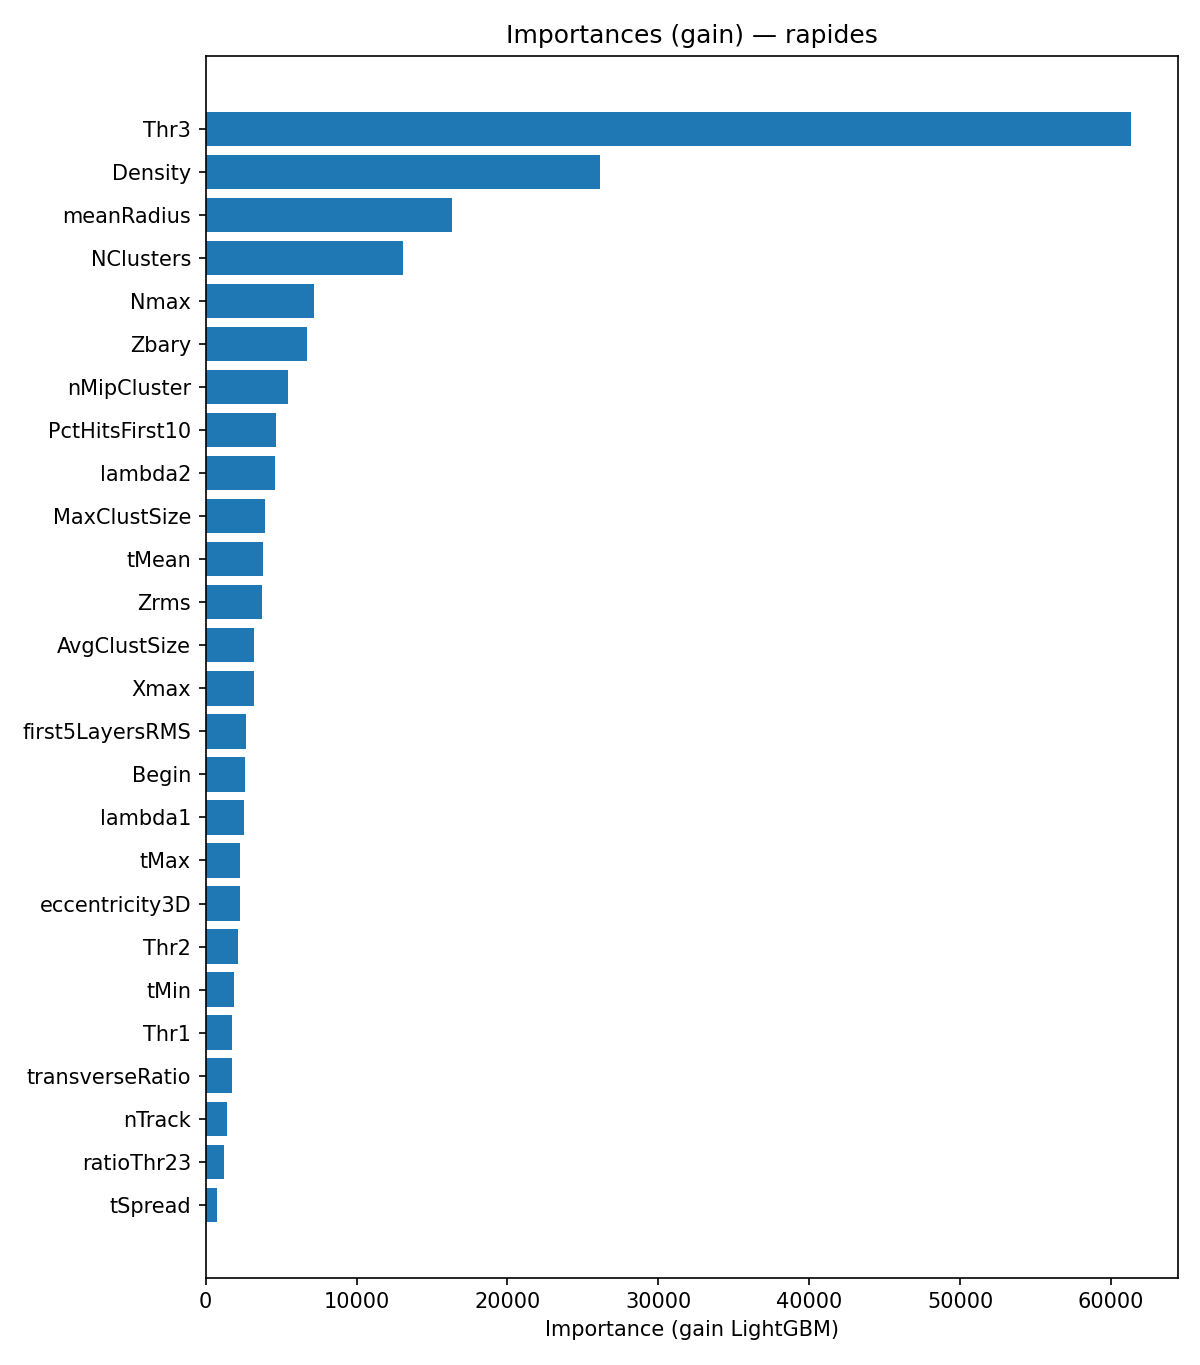
\includegraphics[width=0.90\linewidth,height=0.70\linewidth]{Fig/permutation_importances.png}
  \caption{Importances des variables extraites du modèle LightGBM à partir du gain cumulé.}
  \label{fig:perm-imp}
\end{figure}

\paragraph{Variables dominantes.}

La variable \texttt{Thr3}, correspondant au nombre de hits franchissant le seuil le plus élevé, apparaît comme la plus discriminante, nettement devant les autres. Ce résultat indique que les régions les plus denses de la gerbe jouent un rôle central dans la séparation des espèces. Il suggère que la structure des zones fortement actives constitue une signature importante de l’interaction hadronique.

Les variables \texttt{Density} et \texttt{meanRadius} figurent également parmi les contributions les plus élevées. Elles montrent que la compacité locale et l’extension transverse moyenne de la gerbe sont particulièrement informatives. Le classificateur semble donc s’appuyer fortement sur la morphologie spatiale de l’événement.

Un second groupe d’observables importantes regroupe \texttt{NClusters}, \texttt{Nmax}, \texttt{Zbary}, \texttt{nMipCluster} et \texttt{PctHitsFirst10}. Ces variables traduisent la fragmentation de l’activité, la multiplicité locale et le développement longitudinal de la gerbe, complétant l’information portée par les variables de densité et de compacité.

À l’inverse, les variables temporelles apparaissent ici à un rang plus secondaire. Dans cette configuration, le pouvoir discriminant du modèle est donc principalement porté par les observables décrivant l’intensité locale, la structure spatiale et le développement géométrique des gerbes, davantage que par leur chronologie.

\paragraph{Enseignements pour le PID.}

Cette analyse montre que la séparation des particules repose principalement sur trois familles d’information :
\begin{itemize}
    \item \textbf{la densité locale d’activité}, via \texttt{Thr3} et \texttt{Density} ;
    \item \textbf{la morphologie transverse}, via \texttt{meanRadius} ;
    \item \textbf{la structuration longitudinale et la fragmentation de la gerbe}, via \texttt{Zbary}, \texttt{NClusters} et \texttt{Nmax}.
\end{itemize}

Ces résultats sont cohérents avec la physique des gerbes hadroniques dans un calorimètre hautement granulaire : la compacité, la multiplicité secondaire et la répartition spatiale de l’activité constituent des signatures plus robustes que les seules variables temporelles.

\paragraph{Conséquences pratiques.}

Ces observations suggèrent plusieurs pistes d’amélioration :
\begin{itemize}
    \item réaliser des études d’ablation par groupes de variables (densité, longitudinal, transverse, temps) ;
    \item simplifier le jeu d’entrée en supprimant certaines variables redondantes ;
    \item approfondir l’interprétabilité du modèle à l’aide de méthodes locales telles que SHAP ;
    \item tester explicitement l’impact du retrait complet des variables temporelles.
\end{itemize}

\subsection{Discussion, robustesse et perspectives d'amélioration}

Les résultats obtenus montrent que l’approche par arbres de décision boostés constitue une base solide pour l’identification hadronique dans le SDHCAL. Les performances globales sont satisfaisantes, avec une séparation particulièrement nette des kaons neutres $K^0_L$, tandis que la confusion résiduelle entre protons $p$ et pions $\pi^-$ demeure la principale limitation du classificateur.

L’accuracy globale d’environ $68\,\%$ doit ainsi être interprétée comme un résultat encourageant pour un problème hadronique multiclasse non trivial, mais non comme une performance uniforme sur l’ensemble des classes. L’analyse détaillée par espèce reste donc indispensable.

\paragraph{Interprétation des performances observées.}

La bonne reconnaissance des $K^0_L$ est cohérente avec leur dynamique hadronique spécifique. La présence d’étrangeté, des canaux d’interaction distincts ainsi qu’une production secondaire différente de celle des pions et des protons peuvent modifier la fraction électromagnétique, la compacité locale ou encore le développement longitudinal de la gerbe.

À l’inverse, protons et pions chargés présentent des signatures plus proches. Tous deux interagissent fortement dans l’absorbeur et peuvent produire des cascades secondaires similaires, en particulier lorsque les fluctuations de première interaction dominent. Cette proximité physique se traduit directement par le recouvrement observé dans les distributions de probabilités prédites.

Il est également probable que cette difficulté de séparation dépende de l’énergie incidente : à basse énergie, la faible multiplicité de hits accentue les fluctuations statistiques, tandis qu’à plus haute énergie certaines signatures morphologiques deviennent plus marquées. Une étude différentielle par tranches d’énergie constituerait donc un prolongement naturel.

\paragraph{Robustesse vis-à-vis des effets instrumentaux.}

L’analyse des importances montre que les variables les plus utiles au modèle sont principalement liées à l’activité au seuil élevé, à la densité locale et à la géométrie de la gerbe. Cette hiérarchie apparaît physiquement plausible, mais doit être confirmée dans des conditions instrumentales réalistes.

Il sera notamment nécessaire d’évaluer la stabilité des performances en présence :

\begin{itemize}
    \item d’une résolution temporelle dégradée ;
    \item d’offsets de calibration entre couches ;
    \item de variations des conditions de prise de données ;
    \item d’inefficacités locales ou d’un bruit électronique résiduel ;
    \item de canaux défectueux ou instables.
\end{itemize}

De telles études permettraient de quantifier la sensibilité réelle du classificateur aux non-idéalités expérimentales et de mieux estimer sa transférabilité vers des données réelles.

\paragraph{Réduction et sélection de variables.}

La matrice de corrélation a montré que plusieurs observables transportent une information partiellement redondante, notamment au sein des variables décrivant l’activité globale et la compacité de la gerbe.

Une stratégie raisonnée de sélection de variables pourrait ainsi :

\begin{itemize}
    \item réduire la dimension du problème ;
    \item accélérer l’entraînement ;
    \item limiter la variance statistique ;
    \item améliorer l’interprétabilité physique du modèle.
\end{itemize}

Par exemple, conserver un représentant robuste par groupe corrélé (\texttt{Thr3} ou \texttt{Nmax}, \texttt{Density} ou \texttt{NClusters}, etc.) pourrait suffire sans perte notable de performance.

\paragraph{Améliorations possibles du modèle.}

Bien que LightGBM fournisse déjà de bons résultats, plusieurs axes d’optimisation restent envisageables :

\begin{itemize}
    \item ajustement fin des hyperparamètres (profondeur des arbres, taux d’apprentissage, régularisation L1/L2) ;
    \item pondération spécifique des classes ou des erreurs de classification ;
    \item calibration des probabilités de sortie (Platt scaling, isotonic regression) ;
    \item entraînement conditionné par tranches d’énergie ;
    \item validation croisée sur plusieurs découpages statistiques ;
    \item optimisation directe de métriques équilibrées plutôt que de la seule accuracy.
\end{itemize}

Un apprentissage par intervalles d’énergie pourrait être particulièrement pertinent, les signatures hadroniques évoluant sensiblement entre basse et haute énergie.

Des tests exploratoires de rééquilibrage des classes, notamment via SMOTE, peuvent également être envisagés. Néanmoins, l’intérêt réel de telles méthodes devra être mis en balance avec le risque d’introduire des événements synthétiques peu représentatifs de la physique simulée.

\paragraph{Systématiques liées à la simulation.}

Comme toute approche supervisée entraînée sur simulation, les performances mesurées dépendent du réalisme du modèle physique utilisé pour générer les gerbes hadroniques. Il conviendra donc d’évaluer l’impact :

\begin{itemize}
    \item du choix de la liste de physique utilisée dans Geant4 ;
    \item des paramètres de réponse du détecteur ;
    \item des inefficacités instrumentales ;
    \item de la modélisation temporelle des signaux ;
    \item d’éventuels écarts simulation / données réelles.
\end{itemize}

Une comparaison entre plusieurs configurations de simulation, ainsi qu’une confrontation future aux données expérimentales, permettrait d’estimer l’incertitude systématique associée au classificateur.

\paragraph{Vers des représentations plus fines.}

La principale limite de l’approche actuelle provient de l’utilisation d’un ensemble de variables agrégées. Bien que physiquement motivés, ces descripteurs ne restituent qu’une partie de la richesse spatiale et temporelle des hits bruts du détecteur.

Cela motive naturellement l’exploration de méthodes capables d’exploiter directement la structure native des événements, telles que :

\begin{itemize}
    \item les réseaux convolutifs 3D appliqués à une voxelisation des gerbes ;
    \item les réseaux de neurones graphiques (GNN) construits sur les graphes de hits ;
    \item des approches hybrides combinant descripteurs physiques et représentation brute.
\end{itemize}

\paragraph{Conclusion.}

Le classificateur LightGBM constitue ainsi une solution performante, rapide et interprétable pour l’identification hadronique tabulaire dans le SDHCAL. Ses principales limites actuelles proviennent moins de l’algorithme lui-même que du recouvrement physique entre certaines espèces, en particulier entre pions et protons.

Les progrès futurs passeront principalement par une meilleure maîtrise des effets instrumentaux, une validation approfondie sur conditions réalistes, des études différentielles en énergie et une exploitation plus directe de l’information spatio-temporelle complète des gerbes.

\section{Étude exploratoire : approche GNN}

\paragraph{Motivation.}

L’approche développée jusqu’à présent repose sur un ensemble de descripteurs globaux extraits à partir des hits du détecteur. Cette stratégie fournit une représentation compacte, physiquement interprétable et bien adaptée aux méthodes tabulaires. Elle ne conserve toutefois qu’une partie de l’information spatiale et temporelle contenue dans la topologie fine des gerbes hadroniques.

Or, le SDHCAL est un détecteur hautement granulaire, dont l’un des principaux atouts réside précisément dans la distribution détaillée des hits, couche par couche. Il est donc naturel d’explorer des méthodes capables d’exploiter directement cette information native, sans étape intermédiaire de réduction en variables agrégées.

Dans cette perspective, une étude exploratoire a été menée à l’aide de réseaux de neurones graphiques (\emph{Graph Neural Networks}, GNN).

\paragraph{Principe général.}

Un GNN représente chaque événement sous la forme d’un graphe :

\begin{itemize}
    \item les \textbf{nœuds} correspondent aux hits enregistrés dans le détecteur ;
    \item les \textbf{arêtes} relient des hits voisins ou compatibles selon des critères géométriques et temporels ;
    \item les \textbf{attributs des nœuds} peuvent inclure la position spatiale, le seuil franchi ou le temps associé au hit.
\end{itemize}

Le réseau apprend ensuite à propager et agréger localement l’information entre nœuds connectés afin de construire une représentation globale de la gerbe. Cette approche est particulièrement adaptée aux structures irrégulières, non cartésiennes et peu denses, typiques des calorimètres granulaires.

\paragraph{Cadre de l’étude réalisée.}

Dans le cadre de ce travail, cette méthode a été appliquée à une tâche ciblée de séparation binaire entre pions $\pi$ et protons $p$, sur des événements simulés entre 1 et 100~GeV. Les détails complets de la construction des graphes, du prétraitement des données et de l’architecture utilisée sont présentés en Annexe~\ref{app:gnn}.

Les résultats obtenus doivent être considérés comme préliminaires. Cette étude a été menée en fin de stage et n’a pas donné lieu à une campagne complète de validation systématique ni à l’ensemble des figures de synthèse disponibles pour les approches principales. Elle est donc présentée ici comme une preuve de concept destinée à évaluer le potentiel de cette famille de méthodes.

\paragraph{Résultats obtenus.}

Les premières observations mettent en évidence un rôle déterminant de l’information temporelle.

Lorsque les temps des hits sont conservés avec une précision quasi idéale issue de la simulation (résolution de l’ordre de $\sim10^{-6}$~ns), l’accuracy peut atteindre environ $90\,\%$. Une telle performance traduit principalement l’exploitation d’une information temporelle extrêmement discriminante, liée notamment aux différences de temps de vol entre pions et protons.

Il est important de noter qu’un comportement analogue est observé avec l’approche tabulaire fondée sur BDT lorsque le smearing appliqué à \texttt{tMin} est supprimé. Des performances du même ordre peuvent alors être obtenues. Cela indique que le gain observé provient en grande partie du caractère idéalisé de l’information temporelle disponible en simulation, plutôt que d’une supériorité intrinsèque du GNN sur ce problème de PID.

En revanche, lorsque la résolution temporelle est ramenée à une valeur plus réaliste, de l’ordre de $\sim10$~ps, la performance du GNN redescend autour de $60\,\%$, soit un niveau comparable à celui obtenu avec les méthodes tabulaires classiques.

Dans la configuration étudiée ici, aucun avantage net du GNN n’apparaît donc pour l’identification pion/proton en conditions réalistes.

\paragraph{Interprétation physique.}

La séparation proton/pion repose en partie sur la différence de masse entre les deux particules. À impulsion comparable, celle-ci se traduit par des temps de vol distincts, plus facilement exploitables lorsque la résolution temporelle devient extrêmement fine. Les excellentes performances observées sans smearing reflètent donc principalement l’accès à une information temporelle idéale, difficilement atteignable expérimentalement.

Par ailleurs, la structure locale des premières interactions hadroniques peut également différer subtilement entre les deux espèces. Un GNN est théoriquement capable de capter ce type de corrélations fines entre hits voisins, parfois peu visibles à travers des descripteurs globaux. Néanmoins, dans le cadre présent, cet avantage structurel ne se traduit pas encore par un gain clair dès lors que l’on adopte des conditions temporelles réalistes.

\paragraph{Limites actuelles.}

Cette approche présente plusieurs contraintes :

\begin{itemize}
    \item coût d’entraînement plus élevé que les méthodes tabulaires ;
    \item sensibilité accrue au choix des hyperparamètres ;
    \item besoin de jeux de données volumineux ;
    \item interprétabilité plus limitée ;
    \item dépendance marquée à la définition du graphe (voisinage, connectivité).
\end{itemize}

Dans le cadre présent, il s’agit donc davantage d’une étude exploratoire que d’une alternative immédiatement opérationnelle aux méthodes de boosting.

\paragraph{Perspectives.}

Même si le GNN ne semble pas apporter ici d’amélioration décisive pour le PID, il demeure une approche très prometteuse pour d’autres tâches où la structure détaillée des gerbes joue un rôle plus direct.

En particulier, il paraît potentiellement mieux adapté à la \textbf{reconstruction de l’énergie}, pour laquelle l’exploitation fine de la topologie complète des hits, de leurs corrélations spatiales et de leur organisation locale pourrait fournir un avantage plus marqué que dans une simple classification binaire.

Les GNN pourraient ainsi être particulièrement utiles pour :

\begin{itemize}
    \item la reconstruction d’énergie à partir de la structure complète de la gerbe ;
    \item la reconstruction simultanée PID + énergie ;
    \item les approches de type \emph{Particle Flow} ;
    \item la séparation de gerbes chevauchantes ;
    \item l’exploitation conjointe des informations spatiales et temporelles.
\end{itemize}

Des variantes plus avancées, fondées sur des mécanismes d’attention ou sur l’apprentissage différentiable de la connectivité, pourraient également améliorer les performances futures.

\paragraph{Bilan.}

Cette étude exploratoire montre que les réseaux de neurones graphiques constituent une voie crédible pour exploiter pleinement le potentiel du SDHCAL. Toutefois, dans le cas particulier du PID pion/proton étudié ici, les résultats actuels n’indiquent pas d’avantage clair par rapport au BDT lorsque l’on adopte des conditions temporelles réalistes. En revanche, leur capacité à exploiter directement la structure détaillée des hits en fait une piste particulièrement intéressante pour de futurs travaux consacrés à la reconstruction de l’énergie.


\section{Synthèse}

Ce chapitre a présenté une étude d’identification hadronique dans le SDHCAL fondée sur des méthodes d’apprentissage supervisé appliquées à des échantillons simulés de pions négatifs $\pi^-$, de protons $p$ et de kaons neutres longs $K^0_L$. L’objectif était d’exploiter la richesse spatiale, semi-digitale et géométrique du détecteur afin de distinguer automatiquement ces différentes espèces à partir de la topologie de leurs gerbes.

Parmi les approches testées, les arbres de décision boostés, implémentés via LightGBM, ont offert le meilleur compromis entre performance, rapidité d’entraînement et interprétabilité. Les résultats obtenus sur l’échantillon de test conduisent à une \textbf{accuracy globale d’environ $68\,\%$}. Cette valeur traduit un niveau de performance satisfaisant pour un problème hadronique multiclasse non trivial, mais masque des contrastes importants entre espèces : la séparation des $K^0_L$ apparaît robuste, tandis que la confusion résiduelle entre protons et pions constitue la principale limite actuelle du classificateur.

L’analyse des corrélations entre variables et des importances internes du modèle a permis d’identifier les observables les plus discriminantes. Les variables associées à la densité locale d’activité, au franchissement du seuil élevé (\texttt{Thr3}), à la compacité de la gerbe (\texttt{Density}) ainsi qu’à son extension transverse (\texttt{meanRadius}) apparaissent comme les contributions dominantes. Ce constat est cohérent avec la physique des interactions hadroniques, où la structuration spatiale et l’intensité locale des dépôts constituent des signatures particulièrement informatives.

Ces résultats montrent que le SDHCAL possède un réel potentiel pour l’identification hadronique, y compris dans le cadre d’approches tabulaires relativement simples. Ils soulignent plus largement l’intérêt des calorimètres hautement granulaires, capables de restituer finement la morphologie des gerbes et d’alimenter des méthodes d’analyse avancées.

Ils indiquent également que les limites actuelles proviennent autant de la proximité physique réelle entre certaines espèces hadroniques que du choix de l’algorithme lui-même. Dans le cas pion/proton, le recouvrement partiel des signatures de gerbe rend la séparation intrinsèquement plus délicate.

En parallèle, l’exploration préliminaire d’une approche par réseaux de neurones graphiques a confirmé l’intérêt des représentations construites directement à partir des hits du détecteur. Si aucun gain net n’a été mis en évidence ici pour le PID dans des conditions réalistes, ces méthodes apparaissent comme une piste prometteuse pour exploiter plus complètement la connectivité spatiale des événements, notamment en vue de la reconstruction de l’énergie.

L’ensemble de ces travaux constitue ainsi une base solide pour la suite de ce mémoire, consacrée à un second enjeu majeur de la calorimétrie hadronique : la reconstruction précise de l’énergie incidente.

